\documentclass{standalone}
\ifx\HCode\UnDef\else\def\pgfsysdriver{pgfsys-tex4ht.def}\fi
\usepackage[usenames,dvipsnames,svgnames,table]{xcolor}
\usepackage{tikz}
\usepackage{color}
\usepackage{siunitx}
\usetikzlibrary{arrows,shapes}
\begin{document}
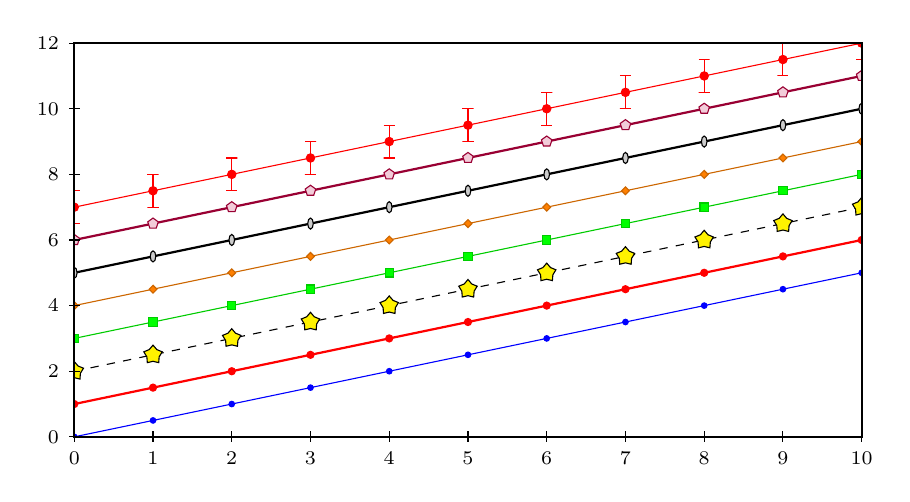
\begin{tikzpicture}
\begin{scope}[]
\pgfpathmoveto{ \pgfpointxy {0.0} {0.0}}
\pgfpathlineto{ \pgfpointxy {10.0} {0.0}}
\pgfpathlineto{ \pgfpointxy {10.0} {5.0}}
\pgfpathlineto{ \pgfpointxy {0.0} {5.0}}
\pgfpathclose
\pgfusepath{  clip, }
\begin{scope}[shift={(0.0,0.0)}]
\pgfsetxvec{\pgfpoint{1.0cm}{0cm}}
\pgfsetyvec{\pgfpoint{0cm}{0.41666666cm}}
\begin{scope}[shift={(0.0,0.0)}]
\begin{scope}[blue]
\pgfpathmoveto{ \pgfpointxy {0.0} {0.0}}
\pgfpathlineto{ \pgfpointxy {1.0} {0.5}}
\pgfpathlineto{ \pgfpointxy {2.0} {1.0}}
\pgfpathlineto{ \pgfpointxy {3.0} {1.5}}
\pgfpathlineto{ \pgfpointxy {4.0} {2.0}}
\pgfpathlineto{ \pgfpointxy {5.0} {2.5}}
\pgfpathlineto{ \pgfpointxy {6.0} {3.0}}
\pgfpathlineto{ \pgfpointxy {7.0} {3.5}}
\pgfpathlineto{ \pgfpointxy {8.0} {4.0}}
\pgfpathlineto{ \pgfpointxy {9.0} {4.5}}
\pgfpathlineto{ \pgfpointxy {10.0} {5.0}}
\pgfusepath{ stroke, }
\end{scope}
\node at (0.0,0.0) [fill=blue,draw=blue,circle,inner sep=0.0pt,minimum width =2.0pt,minimum height=2.0pt] {};
\node at (1.0,0.5) [fill=blue,draw=blue,circle,inner sep=0.0pt,minimum width =2.0pt,minimum height=2.0pt] {};
\node at (2.0,1.0) [fill=blue,draw=blue,circle,inner sep=0.0pt,minimum width =2.0pt,minimum height=2.0pt] {};
\node at (3.0,1.5) [fill=blue,draw=blue,circle,inner sep=0.0pt,minimum width =2.0pt,minimum height=2.0pt] {};
\node at (4.0,2.0) [fill=blue,draw=blue,circle,inner sep=0.0pt,minimum width =2.0pt,minimum height=2.0pt] {};
\node at (5.0,2.5) [fill=blue,draw=blue,circle,inner sep=0.0pt,minimum width =2.0pt,minimum height=2.0pt] {};
\node at (6.0,3.0) [fill=blue,draw=blue,circle,inner sep=0.0pt,minimum width =2.0pt,minimum height=2.0pt] {};
\node at (7.0,3.5) [fill=blue,draw=blue,circle,inner sep=0.0pt,minimum width =2.0pt,minimum height=2.0pt] {};
\node at (8.0,4.0) [fill=blue,draw=blue,circle,inner sep=0.0pt,minimum width =2.0pt,minimum height=2.0pt] {};
\node at (9.0,4.5) [fill=blue,draw=blue,circle,inner sep=0.0pt,minimum width =2.0pt,minimum height=2.0pt] {};
\node at (10.0,5.0) [fill=blue,draw=blue,circle,inner sep=0.0pt,minimum width =2.0pt,minimum height=2.0pt] {};
\begin{scope}[red,thick]
\pgfpathmoveto{ \pgfpointxy {0.0} {1.0}}
\pgfpathlineto{ \pgfpointxy {1.0} {1.5}}
\pgfpathlineto{ \pgfpointxy {2.0} {2.0}}
\pgfpathlineto{ \pgfpointxy {3.0} {2.5}}
\pgfpathlineto{ \pgfpointxy {4.0} {3.0}}
\pgfpathlineto{ \pgfpointxy {5.0} {3.5}}
\pgfpathlineto{ \pgfpointxy {6.0} {4.0}}
\pgfpathlineto{ \pgfpointxy {7.0} {4.5}}
\pgfpathlineto{ \pgfpointxy {8.0} {5.0}}
\pgfpathlineto{ \pgfpointxy {9.0} {5.5}}
\pgfpathlineto{ \pgfpointxy {10.0} {6.0}}
\pgfusepath{ stroke, }
\end{scope}
\node at (0.0,1.0) [fill=red,circle,inner sep=0.0pt,minimum width =3.0pt,minimum height=3.0pt] {};
\node at (1.0,1.5) [fill=red,circle,inner sep=0.0pt,minimum width =3.0pt,minimum height=3.0pt] {};
\node at (2.0,2.0) [fill=red,circle,inner sep=0.0pt,minimum width =3.0pt,minimum height=3.0pt] {};
\node at (3.0,2.5) [fill=red,circle,inner sep=0.0pt,minimum width =3.0pt,minimum height=3.0pt] {};
\node at (4.0,3.0) [fill=red,circle,inner sep=0.0pt,minimum width =3.0pt,minimum height=3.0pt] {};
\node at (5.0,3.5) [fill=red,circle,inner sep=0.0pt,minimum width =3.0pt,minimum height=3.0pt] {};
\node at (6.0,4.0) [fill=red,circle,inner sep=0.0pt,minimum width =3.0pt,minimum height=3.0pt] {};
\node at (7.0,4.5) [fill=red,circle,inner sep=0.0pt,minimum width =3.0pt,minimum height=3.0pt] {};
\node at (8.0,5.0) [fill=red,circle,inner sep=0.0pt,minimum width =3.0pt,minimum height=3.0pt] {};
\node at (9.0,5.5) [fill=red,circle,inner sep=0.0pt,minimum width =3.0pt,minimum height=3.0pt] {};
\node at (10.0,6.0) [fill=red,circle,inner sep=0.0pt,minimum width =3.0pt,minimum height=3.0pt] {};
\begin{scope}[black,dashed]
\pgfpathmoveto{ \pgfpointxy {0.0} {2.0}}
\pgfpathlineto{ \pgfpointxy {1.0} {2.5}}
\pgfpathlineto{ \pgfpointxy {2.0} {3.0}}
\pgfpathlineto{ \pgfpointxy {3.0} {3.5}}
\pgfpathlineto{ \pgfpointxy {4.0} {4.0}}
\pgfpathlineto{ \pgfpointxy {5.0} {4.5}}
\pgfpathlineto{ \pgfpointxy {6.0} {5.0}}
\pgfpathlineto{ \pgfpointxy {7.0} {5.5}}
\pgfpathlineto{ \pgfpointxy {8.0} {6.0}}
\pgfpathlineto{ \pgfpointxy {9.0} {6.5}}
\pgfpathlineto{ \pgfpointxy {10.0} {7.0}}
\pgfusepath{ stroke, }
\end{scope}
\node at (0.0,2.0) [draw=black,fill=yellow,star,star points=5,inner sep=0.0pt,minimum width =7.0pt,minimum height=3.0pt] {};
\node at (1.0,2.5) [draw=black,fill=yellow,star,star points=5,inner sep=0.0pt,minimum width =7.0pt,minimum height=3.0pt] {};
\node at (2.0,3.0) [draw=black,fill=yellow,star,star points=5,inner sep=0.0pt,minimum width =7.0pt,minimum height=3.0pt] {};
\node at (3.0,3.5) [draw=black,fill=yellow,star,star points=5,inner sep=0.0pt,minimum width =7.0pt,minimum height=3.0pt] {};
\node at (4.0,4.0) [draw=black,fill=yellow,star,star points=5,inner sep=0.0pt,minimum width =7.0pt,minimum height=3.0pt] {};
\node at (5.0,4.5) [draw=black,fill=yellow,star,star points=5,inner sep=0.0pt,minimum width =7.0pt,minimum height=3.0pt] {};
\node at (6.0,5.0) [draw=black,fill=yellow,star,star points=5,inner sep=0.0pt,minimum width =7.0pt,minimum height=3.0pt] {};
\node at (7.0,5.5) [draw=black,fill=yellow,star,star points=5,inner sep=0.0pt,minimum width =7.0pt,minimum height=3.0pt] {};
\node at (8.0,6.0) [draw=black,fill=yellow,star,star points=5,inner sep=0.0pt,minimum width =7.0pt,minimum height=3.0pt] {};
\node at (9.0,6.5) [draw=black,fill=yellow,star,star points=5,inner sep=0.0pt,minimum width =7.0pt,minimum height=3.0pt] {};
\node at (10.0,7.0) [draw=black,fill=yellow,star,star points=5,inner sep=0.0pt,minimum width =7.0pt,minimum height=3.0pt] {};
\begin{scope}[green!80!black]
\pgfpathmoveto{ \pgfpointxy {0.0} {3.0}}
\pgfpathlineto{ \pgfpointxy {1.0} {3.5}}
\pgfpathlineto{ \pgfpointxy {2.0} {4.0}}
\pgfpathlineto{ \pgfpointxy {3.0} {4.5}}
\pgfpathlineto{ \pgfpointxy {4.0} {5.0}}
\pgfpathlineto{ \pgfpointxy {5.0} {5.5}}
\pgfpathlineto{ \pgfpointxy {6.0} {6.0}}
\pgfpathlineto{ \pgfpointxy {7.0} {6.5}}
\pgfpathlineto{ \pgfpointxy {8.0} {7.0}}
\pgfpathlineto{ \pgfpointxy {9.0} {7.5}}
\pgfpathlineto{ \pgfpointxy {10.0} {8.0}}
\pgfusepath{ stroke, }
\end{scope}
\node at (0.0,3.0) [draw=green!80!black,fill=green,rectangle,inner sep=0.0pt,minimum width =3.0pt,minimum height=3.0pt] {};
\node at (1.0,3.5) [draw=green!80!black,fill=green,rectangle,inner sep=0.0pt,minimum width =3.0pt,minimum height=3.0pt] {};
\node at (2.0,4.0) [draw=green!80!black,fill=green,rectangle,inner sep=0.0pt,minimum width =3.0pt,minimum height=3.0pt] {};
\node at (3.0,4.5) [draw=green!80!black,fill=green,rectangle,inner sep=0.0pt,minimum width =3.0pt,minimum height=3.0pt] {};
\node at (4.0,5.0) [draw=green!80!black,fill=green,rectangle,inner sep=0.0pt,minimum width =3.0pt,minimum height=3.0pt] {};
\node at (5.0,5.5) [draw=green!80!black,fill=green,rectangle,inner sep=0.0pt,minimum width =3.0pt,minimum height=3.0pt] {};
\node at (6.0,6.0) [draw=green!80!black,fill=green,rectangle,inner sep=0.0pt,minimum width =3.0pt,minimum height=3.0pt] {};
\node at (7.0,6.5) [draw=green!80!black,fill=green,rectangle,inner sep=0.0pt,minimum width =3.0pt,minimum height=3.0pt] {};
\node at (8.0,7.0) [draw=green!80!black,fill=green,rectangle,inner sep=0.0pt,minimum width =3.0pt,minimum height=3.0pt] {};
\node at (9.0,7.5) [draw=green!80!black,fill=green,rectangle,inner sep=0.0pt,minimum width =3.0pt,minimum height=3.0pt] {};
\node at (10.0,8.0) [draw=green!80!black,fill=green,rectangle,inner sep=0.0pt,minimum width =3.0pt,minimum height=3.0pt] {};
\begin{scope}[orange!80!black]
\pgfpathmoveto{ \pgfpointxy {0.0} {4.0}}
\pgfpathlineto{ \pgfpointxy {1.0} {4.5}}
\pgfpathlineto{ \pgfpointxy {2.0} {5.0}}
\pgfpathlineto{ \pgfpointxy {3.0} {5.5}}
\pgfpathlineto{ \pgfpointxy {4.0} {6.0}}
\pgfpathlineto{ \pgfpointxy {5.0} {6.5}}
\pgfpathlineto{ \pgfpointxy {6.0} {7.0}}
\pgfpathlineto{ \pgfpointxy {7.0} {7.5}}
\pgfpathlineto{ \pgfpointxy {8.0} {8.0}}
\pgfpathlineto{ \pgfpointxy {9.0} {8.5}}
\pgfpathlineto{ \pgfpointxy {10.0} {9.0}}
\pgfusepath{ stroke, }
\end{scope}
\node at (0.0,4.0) [draw=orange!80!black,fill=orange,diamond,inner sep=0.0pt,minimum width =3.0pt,minimum height=3.0pt] {};
\node at (1.0,4.5) [draw=orange!80!black,fill=orange,diamond,inner sep=0.0pt,minimum width =3.0pt,minimum height=3.0pt] {};
\node at (2.0,5.0) [draw=orange!80!black,fill=orange,diamond,inner sep=0.0pt,minimum width =3.0pt,minimum height=3.0pt] {};
\node at (3.0,5.5) [draw=orange!80!black,fill=orange,diamond,inner sep=0.0pt,minimum width =3.0pt,minimum height=3.0pt] {};
\node at (4.0,6.0) [draw=orange!80!black,fill=orange,diamond,inner sep=0.0pt,minimum width =3.0pt,minimum height=3.0pt] {};
\node at (5.0,6.5) [draw=orange!80!black,fill=orange,diamond,inner sep=0.0pt,minimum width =3.0pt,minimum height=3.0pt] {};
\node at (6.0,7.0) [draw=orange!80!black,fill=orange,diamond,inner sep=0.0pt,minimum width =3.0pt,minimum height=3.0pt] {};
\node at (7.0,7.5) [draw=orange!80!black,fill=orange,diamond,inner sep=0.0pt,minimum width =3.0pt,minimum height=3.0pt] {};
\node at (8.0,8.0) [draw=orange!80!black,fill=orange,diamond,inner sep=0.0pt,minimum width =3.0pt,minimum height=3.0pt] {};
\node at (9.0,8.5) [draw=orange!80!black,fill=orange,diamond,inner sep=0.0pt,minimum width =3.0pt,minimum height=3.0pt] {};
\node at (10.0,9.0) [draw=orange!80!black,fill=orange,diamond,inner sep=0.0pt,minimum width =3.0pt,minimum height=3.0pt] {};
\begin{scope}[black,thick]
\pgfpathmoveto{ \pgfpointxy {0.0} {5.0}}
\pgfpathlineto{ \pgfpointxy {1.0} {5.5}}
\pgfpathlineto{ \pgfpointxy {2.0} {6.0}}
\pgfpathlineto{ \pgfpointxy {3.0} {6.5}}
\pgfpathlineto{ \pgfpointxy {4.0} {7.0}}
\pgfpathlineto{ \pgfpointxy {5.0} {7.5}}
\pgfpathlineto{ \pgfpointxy {6.0} {8.0}}
\pgfpathlineto{ \pgfpointxy {7.0} {8.5}}
\pgfpathlineto{ \pgfpointxy {8.0} {9.0}}
\pgfpathlineto{ \pgfpointxy {9.0} {9.5}}
\pgfpathlineto{ \pgfpointxy {10.0} {10.0}}
\pgfusepath{ stroke, }
\end{scope}
\node at (0.0,5.0) [draw=black,fill=black!20,ellipse,inner sep=0.0pt,minimum width =2.0pt,minimum height=4.0pt] {};
\node at (1.0,5.5) [draw=black,fill=black!20,ellipse,inner sep=0.0pt,minimum width =2.0pt,minimum height=4.0pt] {};
\node at (2.0,6.0) [draw=black,fill=black!20,ellipse,inner sep=0.0pt,minimum width =2.0pt,minimum height=4.0pt] {};
\node at (3.0,6.5) [draw=black,fill=black!20,ellipse,inner sep=0.0pt,minimum width =2.0pt,minimum height=4.0pt] {};
\node at (4.0,7.0) [draw=black,fill=black!20,ellipse,inner sep=0.0pt,minimum width =2.0pt,minimum height=4.0pt] {};
\node at (5.0,7.5) [draw=black,fill=black!20,ellipse,inner sep=0.0pt,minimum width =2.0pt,minimum height=4.0pt] {};
\node at (6.0,8.0) [draw=black,fill=black!20,ellipse,inner sep=0.0pt,minimum width =2.0pt,minimum height=4.0pt] {};
\node at (7.0,8.5) [draw=black,fill=black!20,ellipse,inner sep=0.0pt,minimum width =2.0pt,minimum height=4.0pt] {};
\node at (8.0,9.0) [draw=black,fill=black!20,ellipse,inner sep=0.0pt,minimum width =2.0pt,minimum height=4.0pt] {};
\node at (9.0,9.5) [draw=black,fill=black!20,ellipse,inner sep=0.0pt,minimum width =2.0pt,minimum height=4.0pt] {};
\node at (10.0,10.0) [draw=black,fill=black!20,ellipse,inner sep=0.0pt,minimum width =2.0pt,minimum height=4.0pt] {};
\begin{scope}[purple!80!black,thick]
\pgfpathmoveto{ \pgfpointxy {0.0} {6.0}}
\pgfpathlineto{ \pgfpointxy {1.0} {6.5}}
\pgfpathlineto{ \pgfpointxy {2.0} {7.0}}
\pgfpathlineto{ \pgfpointxy {3.0} {7.5}}
\pgfpathlineto{ \pgfpointxy {4.0} {8.0}}
\pgfpathlineto{ \pgfpointxy {5.0} {8.5}}
\pgfpathlineto{ \pgfpointxy {6.0} {9.0}}
\pgfpathlineto{ \pgfpointxy {7.0} {9.5}}
\pgfpathlineto{ \pgfpointxy {8.0} {10.0}}
\pgfpathlineto{ \pgfpointxy {9.0} {10.5}}
\pgfpathlineto{ \pgfpointxy {10.0} {11.0}}
\pgfusepath{ stroke, }
\end{scope}
\node at (0.0,6.0) [draw=purple!80!black,fill=purple!20,regular polygon,regular polygon sides=5,inner sep=0.0pt,minimum width =4.0pt,minimum height=4.0pt] {};
\node at (1.0,6.5) [draw=purple!80!black,fill=purple!20,regular polygon,regular polygon sides=5,inner sep=0.0pt,minimum width =4.0pt,minimum height=4.0pt] {};
\node at (2.0,7.0) [draw=purple!80!black,fill=purple!20,regular polygon,regular polygon sides=5,inner sep=0.0pt,minimum width =4.0pt,minimum height=4.0pt] {};
\node at (3.0,7.5) [draw=purple!80!black,fill=purple!20,regular polygon,regular polygon sides=5,inner sep=0.0pt,minimum width =4.0pt,minimum height=4.0pt] {};
\node at (4.0,8.0) [draw=purple!80!black,fill=purple!20,regular polygon,regular polygon sides=5,inner sep=0.0pt,minimum width =4.0pt,minimum height=4.0pt] {};
\node at (5.0,8.5) [draw=purple!80!black,fill=purple!20,regular polygon,regular polygon sides=5,inner sep=0.0pt,minimum width =4.0pt,minimum height=4.0pt] {};
\node at (6.0,9.0) [draw=purple!80!black,fill=purple!20,regular polygon,regular polygon sides=5,inner sep=0.0pt,minimum width =4.0pt,minimum height=4.0pt] {};
\node at (7.0,9.5) [draw=purple!80!black,fill=purple!20,regular polygon,regular polygon sides=5,inner sep=0.0pt,minimum width =4.0pt,minimum height=4.0pt] {};
\node at (8.0,10.0) [draw=purple!80!black,fill=purple!20,regular polygon,regular polygon sides=5,inner sep=0.0pt,minimum width =4.0pt,minimum height=4.0pt] {};
\node at (9.0,10.5) [draw=purple!80!black,fill=purple!20,regular polygon,regular polygon sides=5,inner sep=0.0pt,minimum width =4.0pt,minimum height=4.0pt] {};
\node at (10.0,11.0) [draw=purple!80!black,fill=purple!20,regular polygon,regular polygon sides=5,inner sep=0.0pt,minimum width =4.0pt,minimum height=4.0pt] {};
\begin{scope}[red]
\pgfpathmoveto{ \pgfpointxy {0.0} {7.0}}
\pgfpathlineto{ \pgfpointxy {1.0} {7.5}}
\pgfpathlineto{ \pgfpointxy {2.0} {8.0}}
\pgfpathlineto{ \pgfpointxy {3.0} {8.5}}
\pgfpathlineto{ \pgfpointxy {4.0} {9.0}}
\pgfpathlineto{ \pgfpointxy {5.0} {9.5}}
\pgfpathlineto{ \pgfpointxy {6.0} {10.0}}
\pgfpathlineto{ \pgfpointxy {7.0} {10.5}}
\pgfpathlineto{ \pgfpointxy {8.0} {11.0}}
\pgfpathlineto{ \pgfpointxy {9.0} {11.5}}
\pgfpathlineto{ \pgfpointxy {10.0} {12.0}}
\pgfusepath{ stroke, }
\end{scope}
\begin{scope}[draw=red,fill=red]
\pgfpointadd{\pgfpointxy {0.0} {7.5}} {\pgfpoint{-2pt}{0}}\pgfpathmoveto{ NIL }
\pgfpointadd{\pgfpointxy {0.0} {7.5}} {\pgfpoint{2pt}{0}}\pgfpathlineto{ NIL }
\pgfpointadd{\pgfpointxy {0.0} {7.5}} {\pgfpoint{0pt}{0}}\pgfpathlineto{ NIL }
\pgfpointadd{\pgfpointxy {0.0} {6.5}} {\pgfpoint{0pt}{0}}\pgfpathlineto{ NIL }
\pgfpointadd{\pgfpointxy {0.0} {6.5}} {\pgfpoint{-2pt}{0}}\pgfpathlineto{ NIL }
\pgfpointadd{\pgfpointxy {0.0} {6.5}} {\pgfpoint{2pt}{0}}\pgfpathlineto{ NIL }
\pgfusepath{ stroke, }
\node at (0.0,7.0) [draw=red,fill=red,circle,inner sep=0.0pt,minimum width =3.0pt,minimum height=3.0pt] {};
\end{scope}
\begin{scope}[draw=red,fill=red]
\pgfpointadd{\pgfpointxy {1.0} {8.0}} {\pgfpoint{-2pt}{0}}\pgfpathmoveto{ NIL }
\pgfpointadd{\pgfpointxy {1.0} {8.0}} {\pgfpoint{2pt}{0}}\pgfpathlineto{ NIL }
\pgfpointadd{\pgfpointxy {1.0} {8.0}} {\pgfpoint{0pt}{0}}\pgfpathlineto{ NIL }
\pgfpointadd{\pgfpointxy {1.0} {7.0}} {\pgfpoint{0pt}{0}}\pgfpathlineto{ NIL }
\pgfpointadd{\pgfpointxy {1.0} {7.0}} {\pgfpoint{-2pt}{0}}\pgfpathlineto{ NIL }
\pgfpointadd{\pgfpointxy {1.0} {7.0}} {\pgfpoint{2pt}{0}}\pgfpathlineto{ NIL }
\pgfusepath{ stroke, }
\node at (1.0,7.5) [draw=red,fill=red,circle,inner sep=0.0pt,minimum width =3.0pt,minimum height=3.0pt] {};
\end{scope}
\begin{scope}[draw=red,fill=red]
\pgfpointadd{\pgfpointxy {2.0} {8.5}} {\pgfpoint{-2pt}{0}}\pgfpathmoveto{ NIL }
\pgfpointadd{\pgfpointxy {2.0} {8.5}} {\pgfpoint{2pt}{0}}\pgfpathlineto{ NIL }
\pgfpointadd{\pgfpointxy {2.0} {8.5}} {\pgfpoint{0pt}{0}}\pgfpathlineto{ NIL }
\pgfpointadd{\pgfpointxy {2.0} {7.5}} {\pgfpoint{0pt}{0}}\pgfpathlineto{ NIL }
\pgfpointadd{\pgfpointxy {2.0} {7.5}} {\pgfpoint{-2pt}{0}}\pgfpathlineto{ NIL }
\pgfpointadd{\pgfpointxy {2.0} {7.5}} {\pgfpoint{2pt}{0}}\pgfpathlineto{ NIL }
\pgfusepath{ stroke, }
\node at (2.0,8.0) [draw=red,fill=red,circle,inner sep=0.0pt,minimum width =3.0pt,minimum height=3.0pt] {};
\end{scope}
\begin{scope}[draw=red,fill=red]
\pgfpointadd{\pgfpointxy {3.0} {9.0}} {\pgfpoint{-2pt}{0}}\pgfpathmoveto{ NIL }
\pgfpointadd{\pgfpointxy {3.0} {9.0}} {\pgfpoint{2pt}{0}}\pgfpathlineto{ NIL }
\pgfpointadd{\pgfpointxy {3.0} {9.0}} {\pgfpoint{0pt}{0}}\pgfpathlineto{ NIL }
\pgfpointadd{\pgfpointxy {3.0} {8.0}} {\pgfpoint{0pt}{0}}\pgfpathlineto{ NIL }
\pgfpointadd{\pgfpointxy {3.0} {8.0}} {\pgfpoint{-2pt}{0}}\pgfpathlineto{ NIL }
\pgfpointadd{\pgfpointxy {3.0} {8.0}} {\pgfpoint{2pt}{0}}\pgfpathlineto{ NIL }
\pgfusepath{ stroke, }
\node at (3.0,8.5) [draw=red,fill=red,circle,inner sep=0.0pt,minimum width =3.0pt,minimum height=3.0pt] {};
\end{scope}
\begin{scope}[draw=red,fill=red]
\pgfpointadd{\pgfpointxy {4.0} {9.5}} {\pgfpoint{-2pt}{0}}\pgfpathmoveto{ NIL }
\pgfpointadd{\pgfpointxy {4.0} {9.5}} {\pgfpoint{2pt}{0}}\pgfpathlineto{ NIL }
\pgfpointadd{\pgfpointxy {4.0} {9.5}} {\pgfpoint{0pt}{0}}\pgfpathlineto{ NIL }
\pgfpointadd{\pgfpointxy {4.0} {8.5}} {\pgfpoint{0pt}{0}}\pgfpathlineto{ NIL }
\pgfpointadd{\pgfpointxy {4.0} {8.5}} {\pgfpoint{-2pt}{0}}\pgfpathlineto{ NIL }
\pgfpointadd{\pgfpointxy {4.0} {8.5}} {\pgfpoint{2pt}{0}}\pgfpathlineto{ NIL }
\pgfusepath{ stroke, }
\node at (4.0,9.0) [draw=red,fill=red,circle,inner sep=0.0pt,minimum width =3.0pt,minimum height=3.0pt] {};
\end{scope}
\begin{scope}[draw=red,fill=red]
\pgfpointadd{\pgfpointxy {5.0} {10.0}} {\pgfpoint{-2pt}{0}}\pgfpathmoveto{ NIL }
\pgfpointadd{\pgfpointxy {5.0} {10.0}} {\pgfpoint{2pt}{0}}\pgfpathlineto{ NIL }
\pgfpointadd{\pgfpointxy {5.0} {10.0}} {\pgfpoint{0pt}{0}}\pgfpathlineto{ NIL }
\pgfpointadd{\pgfpointxy {5.0} {9.0}} {\pgfpoint{0pt}{0}}\pgfpathlineto{ NIL }
\pgfpointadd{\pgfpointxy {5.0} {9.0}} {\pgfpoint{-2pt}{0}}\pgfpathlineto{ NIL }
\pgfpointadd{\pgfpointxy {5.0} {9.0}} {\pgfpoint{2pt}{0}}\pgfpathlineto{ NIL }
\pgfusepath{ stroke, }
\node at (5.0,9.5) [draw=red,fill=red,circle,inner sep=0.0pt,minimum width =3.0pt,minimum height=3.0pt] {};
\end{scope}
\begin{scope}[draw=red,fill=red]
\pgfpointadd{\pgfpointxy {6.0} {10.5}} {\pgfpoint{-2pt}{0}}\pgfpathmoveto{ NIL }
\pgfpointadd{\pgfpointxy {6.0} {10.5}} {\pgfpoint{2pt}{0}}\pgfpathlineto{ NIL }
\pgfpointadd{\pgfpointxy {6.0} {10.5}} {\pgfpoint{0pt}{0}}\pgfpathlineto{ NIL }
\pgfpointadd{\pgfpointxy {6.0} {9.5}} {\pgfpoint{0pt}{0}}\pgfpathlineto{ NIL }
\pgfpointadd{\pgfpointxy {6.0} {9.5}} {\pgfpoint{-2pt}{0}}\pgfpathlineto{ NIL }
\pgfpointadd{\pgfpointxy {6.0} {9.5}} {\pgfpoint{2pt}{0}}\pgfpathlineto{ NIL }
\pgfusepath{ stroke, }
\node at (6.0,10.0) [draw=red,fill=red,circle,inner sep=0.0pt,minimum width =3.0pt,minimum height=3.0pt] {};
\end{scope}
\begin{scope}[draw=red,fill=red]
\pgfpointadd{\pgfpointxy {7.0} {11.0}} {\pgfpoint{-2pt}{0}}\pgfpathmoveto{ NIL }
\pgfpointadd{\pgfpointxy {7.0} {11.0}} {\pgfpoint{2pt}{0}}\pgfpathlineto{ NIL }
\pgfpointadd{\pgfpointxy {7.0} {11.0}} {\pgfpoint{0pt}{0}}\pgfpathlineto{ NIL }
\pgfpointadd{\pgfpointxy {7.0} {10.0}} {\pgfpoint{0pt}{0}}\pgfpathlineto{ NIL }
\pgfpointadd{\pgfpointxy {7.0} {10.0}} {\pgfpoint{-2pt}{0}}\pgfpathlineto{ NIL }
\pgfpointadd{\pgfpointxy {7.0} {10.0}} {\pgfpoint{2pt}{0}}\pgfpathlineto{ NIL }
\pgfusepath{ stroke, }
\node at (7.0,10.5) [draw=red,fill=red,circle,inner sep=0.0pt,minimum width =3.0pt,minimum height=3.0pt] {};
\end{scope}
\begin{scope}[draw=red,fill=red]
\pgfpointadd{\pgfpointxy {8.0} {11.5}} {\pgfpoint{-2pt}{0}}\pgfpathmoveto{ NIL }
\pgfpointadd{\pgfpointxy {8.0} {11.5}} {\pgfpoint{2pt}{0}}\pgfpathlineto{ NIL }
\pgfpointadd{\pgfpointxy {8.0} {11.5}} {\pgfpoint{0pt}{0}}\pgfpathlineto{ NIL }
\pgfpointadd{\pgfpointxy {8.0} {10.5}} {\pgfpoint{0pt}{0}}\pgfpathlineto{ NIL }
\pgfpointadd{\pgfpointxy {8.0} {10.5}} {\pgfpoint{-2pt}{0}}\pgfpathlineto{ NIL }
\pgfpointadd{\pgfpointxy {8.0} {10.5}} {\pgfpoint{2pt}{0}}\pgfpathlineto{ NIL }
\pgfusepath{ stroke, }
\node at (8.0,11.0) [draw=red,fill=red,circle,inner sep=0.0pt,minimum width =3.0pt,minimum height=3.0pt] {};
\end{scope}
\begin{scope}[draw=red,fill=red]
\pgfpointadd{\pgfpointxy {9.0} {12.0}} {\pgfpoint{-2pt}{0}}\pgfpathmoveto{ NIL }
\pgfpointadd{\pgfpointxy {9.0} {12.0}} {\pgfpoint{2pt}{0}}\pgfpathlineto{ NIL }
\pgfpointadd{\pgfpointxy {9.0} {12.0}} {\pgfpoint{0pt}{0}}\pgfpathlineto{ NIL }
\pgfpointadd{\pgfpointxy {9.0} {11.0}} {\pgfpoint{0pt}{0}}\pgfpathlineto{ NIL }
\pgfpointadd{\pgfpointxy {9.0} {11.0}} {\pgfpoint{-2pt}{0}}\pgfpathlineto{ NIL }
\pgfpointadd{\pgfpointxy {9.0} {11.0}} {\pgfpoint{2pt}{0}}\pgfpathlineto{ NIL }
\pgfusepath{ stroke, }
\node at (9.0,11.5) [draw=red,fill=red,circle,inner sep=0.0pt,minimum width =3.0pt,minimum height=3.0pt] {};
\end{scope}
\begin{scope}[draw=red,fill=red]
\pgfpointadd{\pgfpointxy {10.0} {12.5}} {\pgfpoint{-2pt}{0}}\pgfpathmoveto{ NIL }
\pgfpointadd{\pgfpointxy {10.0} {12.5}} {\pgfpoint{2pt}{0}}\pgfpathlineto{ NIL }
\pgfpointadd{\pgfpointxy {10.0} {12.5}} {\pgfpoint{0pt}{0}}\pgfpathlineto{ NIL }
\pgfpointadd{\pgfpointxy {10.0} {11.5}} {\pgfpoint{0pt}{0}}\pgfpathlineto{ NIL }
\pgfpointadd{\pgfpointxy {10.0} {11.5}} {\pgfpoint{-2pt}{0}}\pgfpathlineto{ NIL }
\pgfpointadd{\pgfpointxy {10.0} {11.5}} {\pgfpoint{2pt}{0}}\pgfpathlineto{ NIL }
\pgfusepath{ stroke, }
\node at (10.0,12.0) [draw=red,fill=red,circle,inner sep=0.0pt,minimum width =3.0pt,minimum height=3.0pt] {};
\end{scope}
\end{scope}
\pgfsetxvec{\pgfpoint{1cm}{0cm}}
\pgfsetyvec{\pgfpoint{0cm}{1cm}}
\end{scope}
\end{scope}
\begin{scope}[shift={(0.0,0.0)}]
\pgfsetxvec{\pgfpoint{1.0cm}{0cm}}
\pgfsetyvec{\pgfpoint{0cm}{0.41666666cm}}
\begin{scope}[shift={(0.0,0.0)}]
\begin{scope}[thick,black,fill=white]
\pgfpathmoveto{ \pgfpointxy {0.0} {0.0}}
\pgfpathlineto{ \pgfpointxy {10.0} {0.0}}
\pgfpathlineto{ \pgfpointxy {10.0} {12.0}}
\pgfpathlineto{ \pgfpointxy {0.0} {12.0}}
\pgfpathclose
\pgfusepath{ stroke, }
\end{scope}
\begin{scope}[yshift=0cm]
\draw[] [shift={(0.0,0.0)}] (0,2pt) -- (0,-2pt) node[below]{ \scriptsize{\num[round-mode=places,round-precision=0]{0}}};
\draw[] [shift={(1.0,0.0)}] (0,2pt) -- (0,-2pt) node[below]{ \scriptsize{\num[round-mode=places,round-precision=0]{1}}};
\draw[] [shift={(2.0,0.0)}] (0,2pt) -- (0,-2pt) node[below]{ \scriptsize{\num[round-mode=places,round-precision=0]{2}}};
\draw[] [shift={(3.0,0.0)}] (0,2pt) -- (0,-2pt) node[below]{ \scriptsize{\num[round-mode=places,round-precision=0]{3}}};
\draw[] [shift={(4.0,0.0)}] (0,2pt) -- (0,-2pt) node[below]{ \scriptsize{\num[round-mode=places,round-precision=0]{4}}};
\draw[] [shift={(5.0,0.0)}] (0,2pt) -- (0,-2pt) node[below]{ \scriptsize{\num[round-mode=places,round-precision=0]{5}}};
\draw[] [shift={(6.0,0.0)}] (0,2pt) -- (0,-2pt) node[below]{ \scriptsize{\num[round-mode=places,round-precision=0]{6}}};
\draw[] [shift={(7.0,0.0)}] (0,2pt) -- (0,-2pt) node[below]{ \scriptsize{\num[round-mode=places,round-precision=0]{7}}};
\draw[] [shift={(8.0,0.0)}] (0,2pt) -- (0,-2pt) node[below]{ \scriptsize{\num[round-mode=places,round-precision=0]{8}}};
\draw[] [shift={(9.0,0.0)}] (0,2pt) -- (0,-2pt) node[below]{ \scriptsize{\num[round-mode=places,round-precision=0]{9}}};
\draw[] [shift={(10.0,0.0)}] (0,2pt) -- (0,-2pt) node[below]{ \scriptsize{\num[round-mode=places,round-precision=0]{10}}};
\end{scope}
\begin{scope}[xshift=0cm]
\draw[] [shift={(0.0,0.0)}] (2pt,0) -- (-2pt,0) node[left]{ \scriptsize{\num[round-mode=places,round-precision=0]{0}}};
\draw[] [shift={(0.0,2.0)}] (2pt,0) -- (-2pt,0) node[left]{ \scriptsize{\num[round-mode=places,round-precision=0]{2}}};
\draw[] [shift={(0.0,4.0)}] (2pt,0) -- (-2pt,0) node[left]{ \scriptsize{\num[round-mode=places,round-precision=0]{4}}};
\draw[] [shift={(0.0,6.0)}] (2pt,0) -- (-2pt,0) node[left]{ \scriptsize{\num[round-mode=places,round-precision=0]{6}}};
\draw[] [shift={(0.0,8.0)}] (2pt,0) -- (-2pt,0) node[left]{ \scriptsize{\num[round-mode=places,round-precision=0]{8}}};
\draw[] [shift={(0.0,10.0)}] (2pt,0) -- (-2pt,0) node[left]{ \scriptsize{\num[round-mode=places,round-precision=0]{10}}};
\draw[] [shift={(0.0,12.0)}] (2pt,0) -- (-2pt,0) node[left]{ \scriptsize{\num[round-mode=places,round-precision=0]{12}}};
\end{scope}
\end{scope}
\pgfsetxvec{\pgfpoint{1cm}{0cm}}
\pgfsetyvec{\pgfpoint{0cm}{1cm}}
\end{scope}
\end{tikzpicture}
\end{document}
